% ----- Conclusion -----

\section{Conclusion}

As seen in the previous sections, we have been able to implement different
algorithm to solve the Maximum Edge Weight Clique problem. We will be able to
compare the different algorithms and to determine which one is the most
efficient depending on the number of vertices and the connectivity of the graph.
\bigskip

Since the MEWC problem is NP-hard, it is not possible to find a solution in
polynomial time. We have therefore tried to optimize the solution of the problem
by trying to find the most efficient algorithm to solve the problem in the best
way.
\bigskip

Among the different criteria that we will study when comparing these algorithms. We have the \textbf{speed of the results} obtained. This last one is important because the application of the MEWC on different real cases can be subject to certain time constraints. It is obvious that finding the best possible solution would be preferable but as we have seen with the exact, on a large number of vertices, we would need several generations which is not tenable to solve it. This is why we have studied other algorithms that present some alternatives. We are now going to compare them in more detail on the speed of the results obtained. \bigskip

To evaluate this, we will focus on two points: their theoretical complexity but also their execution time in practice that we have done. Note that this comparison is made on randomly generated graphs and therefore presents a general case, but each application case must be seen from a different angle and it is necessary to redo a study. \bigskip

\begin{itemize}
    \item \textbf{Complexity} : As we compare the theorical complexity of the algorithms in general, we obtain : \bigskip
    
    Exact (O($n^2\sqrt[3]{3}^n$)) $>$ Grasp (O($n^6$)) $>$ Local Search (O($n^5$)) $>$ Constructive (O($n^2$)) \bigskip

    We can observe it on the figure \ref{fig:theorical_algorithm_complexity}:

    \begin{figure}[H]
        \centering
        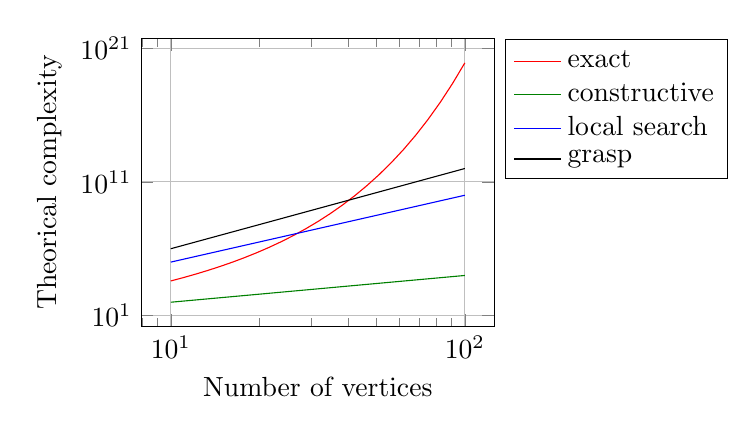
\begin{tikzpicture}
            \begin{loglogaxis}[
                    xlabel = Number of vertices,
                    ylabel = Theorical complexity,
                    legend pos = outer north east,
                    grid = major,
                    width = 0.5\textwidth,
                    legend cell align = {left},
                ]
                \addplot[Red, domain=10:100] {x^2*3^(x/3)};
    
                \addplot[Green, domain=10:100] {x^2};
    
                \addplot[Blue, domain=10:100] {x^5};
    
                \addplot[Black, domain=10:100] {x^6};
    
    
                \addlegendentry{test}
    
                \legend{exact, constructive, local search, grasp}
            \end{loglogaxis}
        \end{tikzpicture}
        \caption{Theorical omplexity of the algorithm in function of the number of vertices.}
        \label{fig:theorical_algorithm_complexity}
    \end{figure}
    
    Since the complexity will vary depending on the connectivity and degeneracy of the graph we will look at the execution time for each graph.
    
    \item \textbf{Execution time} : \bigskip
    
    You can find the execution time in the different experimental parts that we have done before in our report. We get the same results. \bigskip
    
    Exact on figure \ref{fig:exact_time} $>$ Grasp on figure \ref{fig:grasp_time} $>$ Local Search on figure \ref{fig:local_search_time} $>$ Constructive on figure \ref{fig:constructive_time}.
\end{itemize}

Another important criterion to consider is the precision of the results you are looking for, in a real application case, for example let's take our example from figure \ref{fig:applications_example}. You don't necessarily need to get the best possible click, but a slightly worse one will do just fine. The different algorithms we have studied have different levels of expectation in terms of usability results. \bigskip

To evaluate this, we will compare the accuracy of the different algos against the exact one (because it always gives the best result).




\large\textbf{Choice of the algorithm} \newline

After this, we decided to conclude according to the number of vertices of our strating graph :

\begin{itemize}
    \item \textbf{10 - 100 Vertices} : We will use the "Exact" algorithm which allows to give a very precise solution but which is slow.

    \item \textbf{100 + Vertices} : In order to don't wait too long for an answer, we plan to use the "Grasp" algorithm and then the "Local Search" which are certainly less precise but which allows to give an answer in less time.

    \item \textbf{5000 + Vertices} : Finally we will use the "Constructive" algorithm which is the least precise but the fastest and allows to answer in an acceptable time

\end{itemize}

\begin{figure}[H]
    \centering
    \begin{tikzpicture}
        \begin{axis}[
                xlabel = Number of vertices,
                ylabel = \% of solution based on exact,
                legend pos = outer north east,
                grid = major,
                width = 0.5\textwidth,
                legend cell align = {left},
            ]
            \addplot[Red, error bars/.cd, y dir=both, y explicit]
            table[x index=0, y index=1] {experiment_data/accuracy_avg_exact.dat};

            \addplot[Green, error bars/.cd, y dir=both, y explicit]
            table[x index=0, y index=1] {experiment_data/accuracy_avg_constructive_25.dat};

            \addplot[Blue, error bars/.cd, y dir=both, y explicit]
            table[x index=0, y index=1] {experiment_data/accuracy_avg_local_search_25.dat};

            \addplot[Black, error bars/.cd, y dir=both, y explicit]
            table[x index=0, y index=1] {experiment_data/accuracy_avg_grasp_25.dat};

            \addlegendentry{test}

            \legend{exact, constructive, local search, grasp}
        \end{axis}
    \end{tikzpicture}
    \caption{\% of solution based on the exact of the different algorithm for 25\% of connectivity.}
    \label{fig:algorithm_25_time}
\end{figure}

For this experiment, we generated 10 random graphs with 10 to 100 vertices to find an
average \% for 25\% of connectivity. The connectivity is the percentage
of chance that 2 vertices are linked. The results are shown in figure \ref{fig:algorithm_25_time}. At each number of
vertices, an average clique weight is calculated, and converted to \% based on the result obtained with the exact algorithm.
// à martin de détailler

\begin{figure}[H]
    \centering
    \begin{tikzpicture}
        \begin{axis}[
            xlabel = Number of vertices,
            ylabel = \% of solution based on exact,
                legend pos = outer north east,
                grid = major,
                width = 0.5\textwidth,
                legend cell align = {left},
            ]
            \addplot[Red, error bars/.cd, y dir=both, y explicit]
            table[x index=0, y index=1] {experiment_data/accuracy_avg_exact.dat};

            \addplot[Green, error bars/.cd, y dir=both, y explicit]
            table[x index=0, y index=1] {experiment_data/accuracy_avg_constructive_50.dat};

            \addplot[Blue, error bars/.cd, y dir=both, y explicit]
            table[x index=0, y index=1] {experiment_data/accuracy_avg_local_search_50.dat};

            \addplot[Black, error bars/.cd, y dir=both, y explicit]
            table[x index=0, y index=1] {experiment_data/accuracy_avg_grasp_50.dat};

            \addlegendentry{test}

            \legend{exact, constructive, local search, grasp}
        \end{axis}
    \end{tikzpicture}
    \caption{\% of solution based on the exact of the different algorithm for 50\% of connectivity.}
    \label{fig:algorithm_50_time}
\end{figure}

For this experiment, we generated 10 random graphs with 10 to 100 vertices to find an
average \% for 50\% of connectivity. The connectivity is the percentage
of chance that 2 vertices are linked. The results are shown in figure \ref{fig:algorithm_50_time}. At each number of
vertices, an average clique weight is calculated, and converted to \% based on the result obtained with the exact algorithm.
// à martin de détailler

\begin{figure}[H]
    \centering
    \begin{tikzpicture}
        \begin{axis}[
            xlabel = Number of vertices,
            ylabel = \% of solution based on the exact,
                legend pos = outer north east,
                grid = major,
                width = 0.5\textwidth,
                legend cell align = {left},
            ]
            \addplot[Red, error bars/.cd, y dir=both, y explicit]
            table[x index=0, y index=1] {experiment_data/accuracy_avg_exact.dat};

            \addplot[Green, error bars/.cd, y dir=both, y explicit]
            table[x index=0, y index=1] {experiment_data/accuracy_avg_constructive_75.dat};

            \addplot[Blue, error bars/.cd, y dir=both, y explicit]
            table[x index=0, y index=1] {experiment_data/accuracy_avg_local_search_75.dat};

            \addplot[Black, error bars/.cd, y dir=both, y explicit]
            table[x index=0, y index=1] {experiment_data/accuracy_avg_grasp_75.dat};

            \addlegendentry{test}

            \legend{exact, constructive, local search, grasp}
        \end{axis}
    \end{tikzpicture}
    \caption{\% of solution based on the exact of the different algorithm for 75\% of connectivity.}
    \label{fig:algorithm_75_time}
\end{figure}

For this experiment, we generated 10 random graphs with 10 to 100 vertices to find an
average \% of clique weight for 75\% of connectivity. The connectivity is the percentage
of chance that 2 vertices are linked. The results are shown in figure \ref{fig:algorithm_75_time}. At each number of
vertices, an average clique weight is calculated, and converted to \% based on the result obtained with the exact algorithm.
// à martin de détailler

\begin{figure}[H]
    \centering
    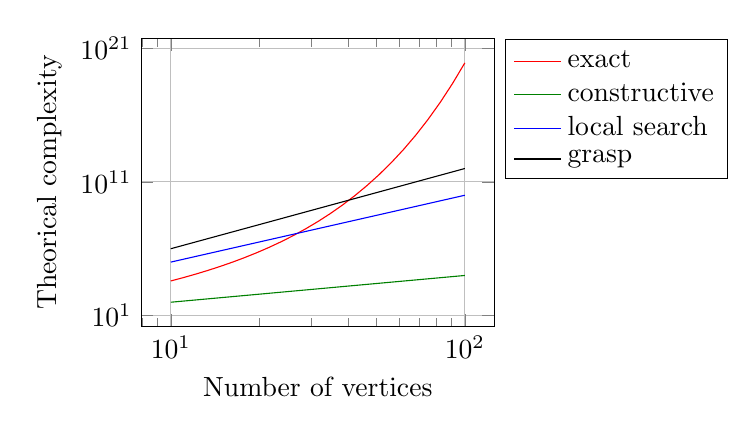
\begin{tikzpicture}
        \begin{loglogaxis}[
                xlabel = Number of vertices,
                ylabel = Theorical complexity,
                legend pos = outer north east,
                grid = major,
                width = 0.5\textwidth,
                legend cell align = {left},
            ]
            \addplot[Red, domain=10:100] {x^2*3^(x/3)};

            \addplot[Green, domain=10:100] {x^2};

            \addplot[Blue, domain=10:100] {x^5};

            \addplot[Black, domain=10:100] {x^6};


            \addlegendentry{test}

            \legend{exact, constructive, local search, grasp}
        \end{loglogaxis}
    \end{tikzpicture}
    \caption{Execution time of the constructive algorithm for different percentages of connectivity.}
    \label{fig:constructive_time}
\end{figure}

In the end, we can conclude that each algorithm has its own advantages and
disadvantages. The exact algorithm is the most accurate, but it is also the most
time-consuming. The constructive algorithm is the fastest, but it is also the
least accurate. The local search algorithm is a good compromise between accuracy
and time. The grasp algorithm is the most accurate of the heuristic approaches,
but it is also the slowest of them.
\bigskip

Generally speaking, the exact algorithm will be employed when the number of
vertices is small, and the heuristic algorithms will be used when the number of
vertices is large.
